\section{Einleitung}


\subsection{Abstract}

Die folgende Dokumentation befasst sich mit den Anforderungen und der Umsetzung eines 'Driver Drowsiness Detection System' Programmes.

Die einzelnen Kapitel befassen sich mit der Herangehensweise und der Umsetzung des Projektes.

Zu Beginn leitet der erste Teil der Ausarbeitung das Thema 'Unfälle durch Müdigkeit am Steuer' ein.

Im nächsten Schritt wird das Ziel beschrieben was durch das Projekt 'Driver Drowsiness Detection System', erreicht werden soll.

Weiterhin werden einige Begriffe erklärt, um das Thema 'Driver Drowsiness Detection System' besser zu erläutern.

Im weiteren Verlauf der Ausarbeitung werden Anwendungsbeispiele zum Thema 'DDD' genannt und 
Unterschiede zu den Projekten der einzelnen Hersteller gezeigt.

Das nächste Kapitel befasst sich mit dem selbst durchgeführten Projekt.

Hier wird beschrieben, was das Projekt macht und welche Programme und Abläufe benötigt werden, 
um das Programm erfolgreich durchzuführen und zu starten.

Am Ende dieser Arbeit wird mit einem Fazit noch einmal resümierend auf die Aufgabe zurückgeschaut, 
aber auch ein Ausblick auf die mögliche Zukunft solcher Programme geworfen. 

\subsection{Thematik}

In Anbetracht der stetig steigenden Unfallrate durch Müdigkeit am Steuer, wurde an dem Projekt 'Driver Drowsiness Detection System' gearbeitet, um für weniger Unfälle zu sorgen.

Zudem soll herausgefunden werden, inwiefern das 'Driver Drowsiness Detection System' im Alltag für mehr Sicherheit sorgen kann. 

So soll das Projekt an mehreren Nutzern getestet- und ihr Verhalten analysiert werden.

Geplant ist es, mit dem 'Driver Drowsiness Detection System' Unfälle auf den Straßen zu verhindern.

In den Jahren, 2012-2019 (Österreich), waren es durchschnittlich 500 Unfälle mit Personenschaden, 
dabei starben im Schnitt 14 Menschen.

Im Jahr 2020 (Österreich), gab es einen deutlichen Rückgang von durchschnittlich 268 Unfällen und 6 davon endeten tödlich. 

Wegen den aktuellen Corona-Maßnahmen wurde das Fahren für Pendler und Urlaubsfahrten, stark eingeschränkt. 

Somit nahm auch die Unfallzahl stark ab.

Auch durch das vermehrte Einsetzen von einem 'Aufmerksamkeits-Assistenten', wird Jahr für Jahr die Unfallrate geringer.\cite{b6}

\subsection{Aufgabe}

\begin{figure}[htbp]
  \centering
     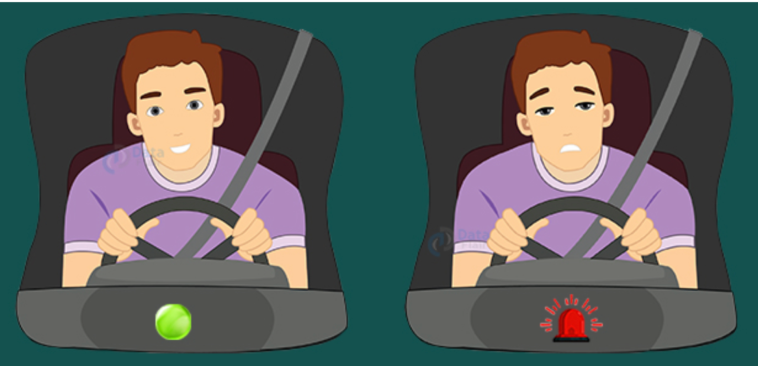
\includegraphics[width=0.40\textwidth]{Fahrer.png}
     \caption{Driver Drowsiness Detection}
\end{figure}

Die Aufgabe des Projektes stellt das Bild, 'Driver Drowsiness Detection' dar.

Auf dem Bild ist eine Person zu sehen, die in zwei unterschiedlichen Positionen hinter einem Lenkrad sitzt.

Auf dem linken Bild ist zu erkenne, dass die Person munter und entspannt hinterm dem Steuer sitzt.

Zudem zeigt eine grüne Lampe an, dass bei der linken Situation keine Probleme/Gefahren entstehen.

Auf dem rechten Bild, ist die selbe Person dargestellt, jedoch leuchtet hier eine rote Warnlampe.

Auch sieht man der Person an, dass sie müde oder angespannt ist.

Die Person hat ihre Mundwinkel nach unten gerichtet und die Augen sind leicht geschlossen.

Die Aufgabe besteht darin, zu erkennen wann die Person fahrtüchtig ist (grüne Lampe bedeutet Augen offen) oder nicht fahrtüchtig (rote Lampe bedeutet Augen geschlossen).


\subsection{Ziel}
Das Ziel des Projektes ist, zu erkennen, ob eine Person hinter dem Steuer fahrtüchtig oder nicht fahrtüchtig ist. 

Um das Ziel umzusetzen, wird ein Programm benötigt welches erkennen soll, wann die Person ihre Augen offen oder geschlossen hat.

So soll das Programm über eine 'Webcam' das Gesicht der Person erkennen und die Werte einlesen.

Mit den Werten soll entschieden werden, ob die Person weiterfahren darf oder eine Pause einlegen muss.

Dies soll über ein rotes Warnsignal und Tonsignal dem Fahrer angezeigt werden.
\newline
\newline